\documentclass{article}
\usepackage[margin=1in]{geometry}
\usepackage{amsmath}
\usepackage{graphicx}
\usepackage{siunitx}
\usepackage{listings}
\usepackage{xcolor}
\usepackage{hyperref}
\definecolor{mygreen}{rgb}{0,0.6,0}
\definecolor{mygray}{rgb}{0.5,0.5,0.5}
\definecolor{mymauve}{rgb}{0.58,0,0.82}

\lstset{ %
  backgroundcolor=\color{white},   % choose the background color; you must add \usepackage{color} or \usepackage{xcolor}
  basicstyle=\scriptsize\ttfamily,    % the size of the fonts that are used for the code
  breakatwhitespace=false,         % sets if automatic breaks should only happen at whitespace
  breaklines=true,                 % sets automatic line breaking
  captionpos=b,                    % sets the caption-position to bottom
  commentstyle=\color{mygreen},    % comment style
  deletekeywords={},            % if you want to delete keywords from the given language
  escapeinside={\%*}{*)},          % if you want to add LaTeX within your code
  extendedchars=true,              % lets you use non-ASCII characters; for 8-bits encodings only, does not work with UTF-8
  frame=shadowbox,                    % adds a frame around the code
%  framexleftmarign=5mm,
  xleftmargin=10pt,
  xrightmargin=10pt,
  rulesepcolor=\color{gray},
  keywordstyle=\color{blue},       % keyword style
  language=Octave,                 % the language of the code
  morekeywords={*,...,fit,predint,export\_fig},            % if you want to add more keywords to the set
%  numbers=left,                    % where to put the line-numbers; possible values are (none, left, right)
  numbers=none,
  numbersep=5pt,                   % how far the line-numbers are from the code
  numberstyle=\tiny\color{mygray}, % the style that is used for the line-numbers
  rulecolor=\color{black},         % if not set, the frame-color may be changed on line-breaks within not-black text (e.g. comments (green here))
  showspaces=false,                % show spaces everywhere adding particular underscores; it overrides 'showstringspaces'
  showstringspaces=false,          % underline spaces within strings only
  showtabs=false,                  % show tabs within strings adding particular underscores
  stepnumber=1,                    % the step between two line-numbers. If it's 1, each line will be numbered
  stringstyle=\color{mymauve},     % string literal style
  tabsize=4,                       % sets default tabsize to 4 spaces
  caption=\lstname                   % show the filename of files included with \lstinputlisting; also try caption instead of title
}


\title{1.723 HW7}
\author{Sachith  Dunatunga}

\begin{document}
\newcommand{\deriv}[2]{\frac{\partial #1}{ \partial #2}}
\newcommand{\nderiv}[3]{\frac{\partial^{#3} #1}{ \partial #2^{#3}}}
\newcommand{\dx}[1]{\deriv{#1}{x}}
\newcommand{\taylorexpf}[3]{#1_{#2} + \left(#3 \right) \dx{#1}\biggr\rvert_{#2} + \frac{1}{2}\left(#3 \right)^2 \nderiv{#1}{x}{2}\biggr\rvert_{#2} + \frac{1}{6}\left(#3 \right)^3\nderiv{#1}{x}{3}\biggr\rvert_{#2} + \frac{1}{24}\left(#3 \right)^4\nderiv{#1}{x}{4}\biggr\rvert_{#2} + O(h^5)}
\maketitle

\section{Problem 1}
\begin{enumerate}
\item
In order to determine the coefficients of the points in the stencil near the boundary, we first write the taylor expansions for a few points given by
\begin{align}
u_{j-3} &= \taylorexpf{u}{j}{-3h} \\
u_{j-2} &= \taylorexpf{u}{j}{-2h} \\
u_{j-1} &= \taylorexpf{u}{j}{-1h} \\
u_j &= u_j \\
u_{j+1} &= \taylorexpf{u}{j}{1h} \\
u_{j+2} &= \taylorexpf{u}{j}{2h} \\
u_{j+3} &= \taylorexpf{u}{j}{3h}.
\end{align}

We note that this can be written as a matrix between the scaled deriative vector $\mathbf{\tilde{u}'}$ and the vector on the grid $\mathbf{u}$.
We scale the derivatives by a factor of $h$ per derivative, so the first term of $\mathbf{\tilde{u}'}$ is just the zeroth derivative $u_j$, the second term is $h u'_j$, the third is $h^2 u''_j$, etc.
As an example, if we are looking at the leftmost point, we do not have points to the left, and in the matrix vector equation $\mathbf{u} = \mathbf{A} \mathbf{\tilde{u}'}$ $\mathbf{A}$ is given by
\begin{align}
\mathbf{A} = \begin{bmatrix}
1 & 3 & \frac{9}{2} & \frac{9}{2} \\
1 & 2 & 2 & \frac{4}{3} \\
1 & 1 & \frac{1}{2} & \frac{1}{6} \\
1 & 0 & 0 & 0
\end{bmatrix}.
\end{align}

However, note that we wish to determine the coefficients of the components of $\mathbf{u}$ to give a specific vector $\mathbf{\tilde{u}'}$ instead of using derivative information to reconstruct grid point values.
This means we need to solve $\mathbf{A}^T \mathbf{c} = \mathbf{b}$ for $\mathbf{c}$, where $\mathbf{c}$ is the vector of coefficients for the grid points and $\mathbf{b}$ is the vector which represents the combination of derivatives desired (for the first derivative, this becomes $[0, 1, 0, 0]^T$).

For this leftmost point, the coefficient vector becomes $\frac{1}{6}[11,-18,9,-2]$; this translates to the stencil
\begin{align}
w_0 = \frac{-11 u_0 + 18 u_1 - 9 u_2 + 2 u_3 }{6h}.
\end{align}

The process may be repeated for the second-leftmost point, yielding the stencil
\begin{align}
w_1 = \frac{- 2 u_0 - 3 u_1 + 6 u_2 - u_3}{6h}.
\end{align}

Similarly, the second-rightmost point and rightmost points have the stencils
\begin{align}
w_{N-1} &= \frac{u_{N-3} - 6 u_{N-2} + 3 u_{N-1} +  2 u_{N}}{6h} \\
w_{N} &= \frac{- 2 u_{N-3} + 9 u_{N-2} - 18 u_{N-1} + 11 u_{N}}{6h}
\end{align}
respectively.

\item
The code is shown in listing \ref{code:p1} and listing \ref{code:p1m}.
Running the code on the sample function $u(x) = \exp(\sin (2 \pi x))$ over various N gives the convergence plot shown in \ref{fig:p1}.
As expected, it is fourth order accurate (although the boundaries are only 3rd order accurate, the function is smooth enough that the boundaries don't contribute too much error).
\begin{figure}[!ht]
\centering
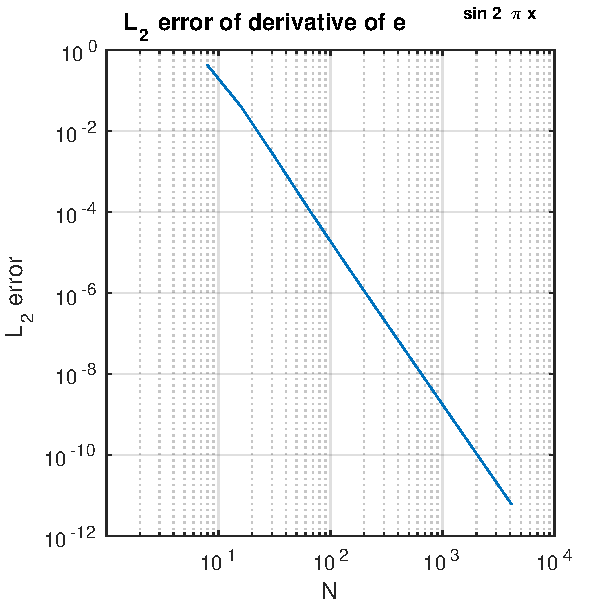
\includegraphics[scale=1]{p1err.pdf}
\caption{The $L_2$ error of the numerically calculated derivative compared to the analytical solution. This error converges at fourth order. The $L_2$ error is calculated by $\frac{1}{N} \sqrt{ \sum{(u'^{approx}_j - u'^{exact}_j)^2}}$.}
\label{fig:p1}
\end{figure}
\end{enumerate}

\section{Problem 2}
\begin{enumerate}

\item
We use the same framework as before to determine the coefficients for the stencil for the centered fourth-order second derviative operator, given by
\begin{align}
w_j = \frac{-u_{j-2} + 16 u_{j-1} -30 u_j + 16 u_{j+1} - u_{j+2}}{12h^2}.
\end{align}
To verify this is indeed fourth order, we can simply expand the terms, which is quite tedious.
Instead, we note that, by construction, the approximation is at least third order (the form of the b vector is [0, 0, 1, 0, 0], and we eventually divide by $h^2$).
However, because of symmetry in the coefficients, the term containing $\nderiv{u}{x}{5}$ is also set to 0, so the largest term is $\nderiv{u}{x}{6} O(h^4)$ after collecting terms and dividing.

\item
The code is shown in listing \ref{code:p2} and listing \ref{code:p2m}.
The errors are plotted in figure \ref{fig:p2} when using the function $u(x) = \exp(\sin(x) \sin(x))$. As expected, the error converges at fourth order.
\begin{figure}[!ht]
\centering
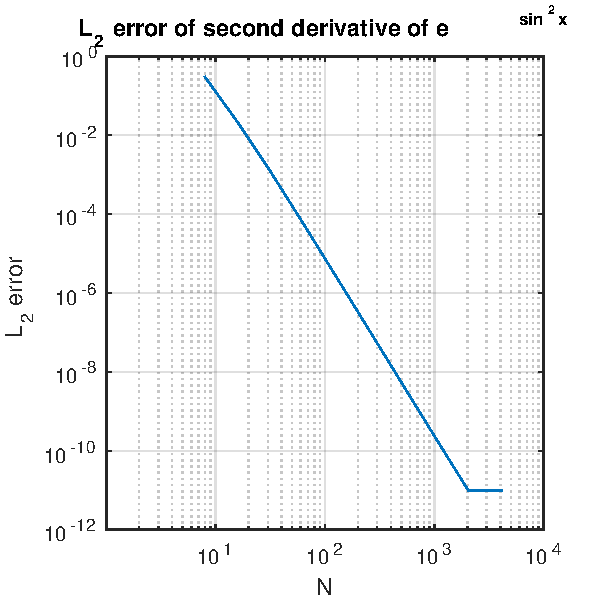
\includegraphics[scale=1]{p2err.pdf}
\caption{The $L_2$ error of the numerically calculated derivative compared to the analytical solution. This error converges at fourth order. $L_2$ error is defined as before.}
\label{fig:p2}
\end{figure}

\item
The same code is used as before.
If we instead use the function $u(x) = \exp(\sin(x) |\sin(x)|)$, the error converges only at first order, as seen in figure \ref{fig:p2abs}.
This is because the derivative is not continuous, which can be seen from the analytical solution
\begin{align}
\nderiv{u}{x}{2} = \exp(\sin(x) |\sin(x)|) \left( 2 \cos(2 x) \mathrm{sign}(\sin(x)) + \sin^2(2 x) \right).
\end{align}
\begin{figure}[!ht]
\centering
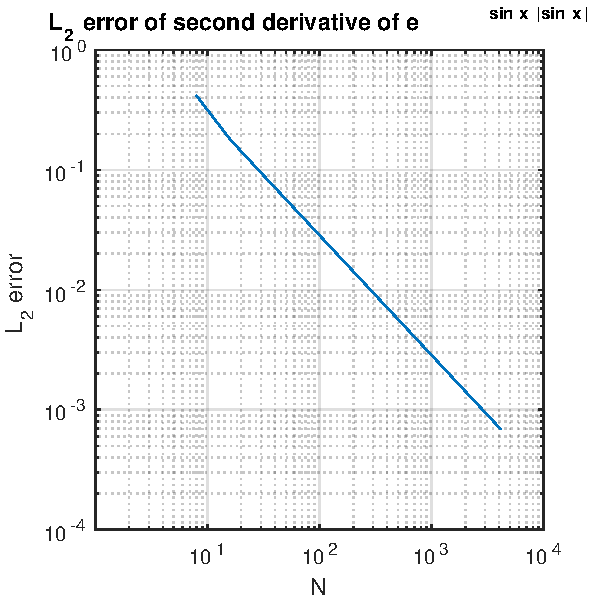
\includegraphics[scale=1]{p2errabs.pdf}
\caption{The $L_2$ error of the numerically calculated derivative compared to the analytical solution. This error converges only at first order, due to a discontinuous derivative. $L_2$ error is defined as before.}
\label{fig:p2abs}
\end{figure}
\end{enumerate}

\clearpage
\appendix
\section{Code}
\lstinputlisting[label=code:p1]{p1.m}
\lstinputlisting[label=code:p1m]{p1_fdmatrix.m}
\lstinputlisting[label=code:p2]{p2.m}
\lstinputlisting[label=code:p2m]{p2_fdmatrix.m}

\end{document}
